% macro_usage_guide.tex
% Beknopte handleiding voor school-macros

\documentclass[a4paper,11pt]{article}
\usepackage{school-macros}
\usepackage{siunitx}
\sisetup{per-mode=symbol}

\title{School Macros: Snelgids}
\author{}
\date{\today}

\begin{document}

\maketitle
\tableofcontents
\section{Essentiële Boxen}

Vier simpele boxen voor je documenten:

\begin{examenbox}
Gebruik deze voor examenvragen en belangrijke tips.
\end{examenbox}

\begin{warningbox}
Voor kritische aandachtspunten en waarschuwingen.
\end{warningbox}

\begin{theorieblok}
Voor theoretische uitleg en definities.
\end{theorieblok}

\begin{oefenblok}
Voor oefeningen en voorbeelden.
\end{oefenblok}

\section{Formules}

Gebruik \verb|\frm| voor belangrijke formules. Deze komen automatisch in het formularium:

\frm{Kinetische Energie}
    {E_k = \frac{1}{2}mv^2}
    {Waarbij $m$ de massa [kg] en $v$ de snelheid [m/s] is.}

\section{Symbolen}

Bij eerste gebruik toont \verb|\sym| een uitleg. Daarna alleen het symbool:

\sym{f}{Frequentie}{Hz}

Later in de tekst: $f = 50$ Hz (gewoon het symbool gebruiken).

\section{Figuren}

\verb|\fig[breedte]{pad}{onderschrift}{label}|

Voorbeeld: \verb|\fig[0.6\linewidth]{image.png}{Een grafiek}{fig:grafiek}|

\section{Nuttige Wiskunde}

\subsection{Afgeleiden}
\begin{itemize}
    \item \verb|\dd{y}{x}| voor $\displaystyle\dd{y}{x}$
    \item \verb|\pd{f}{x}| voor $\displaystyle\pd{f}{x}$
    \item \verb|\dx, \dy, \dt| voor integralen: $\int f(x) \, \dx$
\end{itemize}

\subsection{Vectoren}
\begin{itemize}
    \item \verb|\vec{v}| geeft $\vec{v}$
    \item \verb|\uvec{n}| geeft $\uvec{n}$ (eenheidsvector)
\end{itemize}

\subsection{Haakjes}
\begin{itemize}
    \item \verb|\abs{x}| voor $\abs{x}$
    \item \verb|\norm{v}| voor $\norm{v}$
    \item \verb|\paren{...}|, \verb|\bracket{...}|, \verb|\curlybrace{...}|
\end{itemize}

\subsection{Snelle Breuken}
\verb|\half|, \verb|\third|, \verb|\quarter| geeft $\half$, $\third$, $\quarter$

\section{Eenheden}

Met siunitx package:
\begin{itemize}
    \item \verb|\SI{100}{\km}| → \SI{100}{\km}
    \item \verb|\SI{25}{\degC}| → \SI{25}{\degC}
    \item \verb|\SI{9.81}{\ms}| → \SI{9.81}{\ms}
\end{itemize}

Shortcuts: \verb|\km, \kmh, \ms, \degC, \kW, \MW, \kPa, \MPa|

\section{Nadruk}

\begin{itemize}
    \item \verb|\concept{...}| voor \concept{nieuwe begrippen}
    \item \verb|\belangrijk{...}| voor \belangrijk{belangrijke zaken}
\end{itemize}

\section{Lijsten}

\subsection{Opsomming (itemize)}
\begin{itemize}
    \item Eerste punt
    \item Tweede punt
    \item Geneste lijsten:
    \begin{itemize}
        \item Sub-punt A
        \item Sub-punt B
    \end{itemize}
\end{itemize}

\subsection{Genummerd (enumerate)}
\begin{enumerate}
    \item Eerste stap
    \item Tweede stap
    \item Derde stap
\end{enumerate}

\subsection{Beschrijving (description)}
\begin{description}
    \item[Snelheid] Afgelegde afstand per tijdseenheid
    \item[Versnelling] Verandering van snelheid per tijdseenheid
\end{description}

\section{Tabellen}

Gebruik \texttt{booktabs} voor professionele tabellen:

\begin{table}[H]
\centering
\caption{Materiaaleigenschappen}
\begin{tabular}{lcc}
\toprule
\textbf{Materiaal} & \textbf{Dichtheid} & \textbf{E-modulus} \\
 & [\si{\kg\per\cubic\meter}] & [\si{\giga\pascal}] \\
\midrule
Staal & 7850 & 210 \\
Aluminium & 2700 & 70 \\
Beton & 2400 & 30 \\
\bottomrule
\end{tabular}
\end{table}

\section{Grafieken}

\subsection{Functie Plot}
\begin{center}
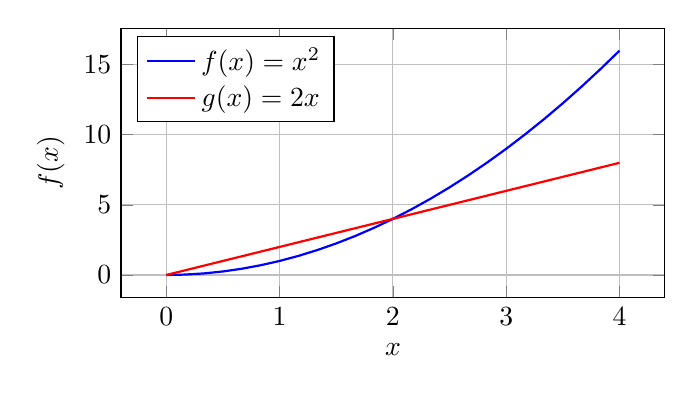
\begin{tikzpicture}
\begin{axis}[
    width=0.7\linewidth,
    height=5cm,
    xlabel={$x$},
    ylabel={$f(x)$},
    grid=major,
    legend pos=north west
]
\addplot[blue, thick, domain=0:4] {x^2};
\addlegendentry{$f(x) = x^2$}
\addplot[red, thick, domain=0:4] {2*x};
\addlegendentry{$g(x) = 2x$}
\end{axis}
\end{tikzpicture}
\end{center}

\subsection{Data Plot}
\begin{center}
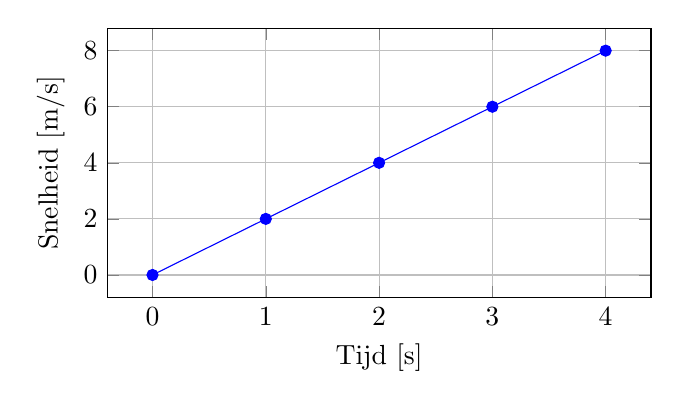
\begin{tikzpicture}
\begin{axis}[
    width=0.7\linewidth,
    height=5cm,
    xlabel={Tijd [s]},
    ylabel={Snelheid [m/s]},
    grid=major
]
\addplot[mark=*, blue] coordinates {
    (0,0) (1,2) (2,4) (3,6) (4,8)
};
\end{axis}
\end{tikzpicture}
\end{center}

\subsection{Eenvoudig Diagram}
\begin{center}
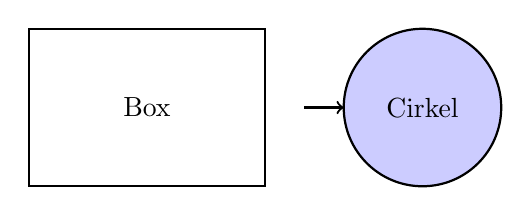
\begin{tikzpicture}
% Rechthoek
\draw[thick] (0,0) rectangle (3,2);
% Cirkel
\draw[thick, fill=blue!20] (5,1) circle (1);
% Pijl
\draw[->, thick] (3.5,1) -- (4,1);
% Tekst
\node at (1.5,1) {Box};
\node at (5,1) {Cirkel};
\end{tikzpicture}
\end{center}

\section{Geavanceerde Layout}

\subsection{Tekst naast Figuur}
Wil je een afbeelding naast tekst plaatsen? Gebruik twee `minipage` omgevingen naast elkaar.

\begin{figure}[H]
    \centering
    \begin{minipage}{0.6\textwidth}
        \textbf{Uitleg bij de figuur:}\\
        Soms is een figuur te smal om de hele breedte te vullen, of wil je direct uitleg ernaast geven.
        
        Door de pagina op te splitsen in twee blokken (minipages) kun je tekst en beeld naast elkaar zetten.
        Let op dat de breedtes samen niet meer dan \texttt{1.0\\textwidth} zijn (hier 0.6 en 0.35).
    \end{minipage}%
    \hfill
    \begin{minipage}{0.35\textwidth}
        \centering
        \includegraphics[width=\linewidth]{image1.png}
        \caption{Kleine figuur}
    \end{minipage}
\end{figure}

\subsection{Tabellen met veel tekst}
Gebruik \texttt{tabularx} als je een tabel wilt die de hele paginabreedte vult en waarbij de tekst automatisch naar de volgende regel gaat. Gebruik \texttt{X} voor de kolom die zich moet aanpassen.

\begin{table}[H]
    \centering
    \caption{Voorbeeld met lange tekst}
    \begin{tabularx}{\linewidth}{l X l}
        \toprule
        \textbf{Begrip} & \textbf{Lange Omschrijving} & \textbf{Categorie} \\
        \midrule
        Marketing & Het proces waarmee bedrijven waarde creëren voor klanten en sterke klantrelaties opbouwen om in ruil daarvoor waarde van klanten te verkrijgen. & Business \\
        \addlinespace
        Inflatie & Een algemene stijging van het prijspeil van goederen en diensten in een economie over een bepaalde periode. & Economie \\
        \bottomrule
    \end{tabularx}
\end{table}

\subsection{Layout Tips}
\begin{itemize}
    \item \textbf{Witruimte:} LaTeX regelt witruimte meestal goed. Gebruik \verb|\vspace{1cm}| alleen als het echt moet.
    \item \textbf{Nieuwe pagina:}
    \begin{itemize}
        \item \verb|\newpage|: Start direct een nieuwe pagina.
        \item \verb|\clearpage|: Start een nieuwe pagina én plaatst alle nog "zwevende" figuren/tabellen direct. Dit voorkomt dat figuren opschuiven naar het einde van het hoofdstuk.
    \end{itemize}
    \item \textbf{Zwevende elementen:} Gebruik \texttt{[H]} (van het \texttt{float} package) als je een figuur of tabel \textit{precies hier} wilt dwingen, maar wees er zuinig mee. LaTeX plaatst ze vaak beter zelf bovenaan \texttt{[t]} of onderaan \texttt{[b]}.
\end{itemize}

\section{Workflow}

\subsection{Typisch Document}
\begin{verbatim}
\documentclass[a4paper,11pt]{report}
\usepackage{school-macros}
\usepackage{siunitx}

\begin{document}

\chapter{Hoofdstuk}

\frm{Label}{formule}{uitleg}
\sym{x}{Naam}{Eenheid}

\begin{examenbox}
Belangrijke tip...
\end{examenbox}

\begin{oefenblok}
Oefening...
\end{oefenblok}

\appendix
\printsymbols
\printformularium

\end{document}
\end{verbatim}

\subsection{Belangrijk}
\begin{enumerate}
    \item Compileer \textbf{tweemaal} voor formularium en symbolenlijst
    \item Gebruik \verb|\frm| voor alle belangrijke formules
    \item Gebruik \verb|\sym| bij eerste vermelding van symbolen
    \item Eenheden altijd via \verb|\SI{waarde}{eenheid}|
\end{enumerate}

\appendix
\section*{Symbolenlijst}
\printsymbols

\section*{Formularium}
\printformularium

\end{document}
